\documentclass{article}
\usepackage{graphicx}				
\usepackage{mathtools}	
\usepackage{hyperref}

\begin{document}
\title{Big programming exercise, task 16: Arcsine function}
\author{Jedrzej Jawor}
\date{}
\maketitle

\section{Introduction}
This report aims to implement the arcsine function using numerical root-finding routines from the GNU scientific library (GSL).

\section{Theory}
Root finding routines are mathematical routines that find the roots of functions. A root of a function $f(x)$ is the value 
of $x$ at which $f(x)$ is equal to 0.
\\
A system of equations can be recast as a root finding problem. Given two functions of x: $f(x)$ and $g(x)$ equal to eachother 
\cite{wikiroots}.
\begin{equation}
\label{eq:1}
f(x)=g(x) \Rightarrow h(x)=f(x)-g(x).
\end{equation}

Finding the solution of the equation is the same as finding the roots of $h(x)$.
\\
In this project I specifficly look at the arcsine function.
\begin{equation}
\label{eq:asin}
a(x)=arcsin(x).
\end{equation}
This function can be recast as a root finding problem by taking the sine on both sides and subtracting one side:

\begin{equation}
\label{eq:asin2}
sin(a(x))=sin(arcsin(x)) = x \Rightarrow 0 = h(x) = x-sin(a(x))
\end{equation}

The value of a(x) can now be computed numericly by finding the values of $a(x)$ that correspond to the roots of $h(x)$ 
for different values of x.

\section{Numerical solution}
I order to find the roots of equation \ref{eq:asin2} I use the multidimensional root finding algorythms from GSL \cite{GSL}.

Note that this is a one-dimensional problem and can be treated using the one-dimensional root-finding algorythms from GSL. 
I chose to work with the multidimensional algorythms as I am more familiar with them.

I used the "Hybrid" algorythm, casting equation \ref{eq:asin2} with x as a parameter and $a(x)$ as the unknown to be found. 
The values of $a(x)$ corresponding to the roots of the equation were then found for different values of x 
ranging from $x=-1$ to $x=1$ with step size $dx=0.05$.
\\
The found values of $a(x)$ are plotted as function of x. 
I also plot the built-in arcsin function from the math library "math.h" as refernce and compare it to the numerical solution.
The plot can be seen on figure \ref{fig:1}  


\begin{figure}[h]
\label{fig:1}
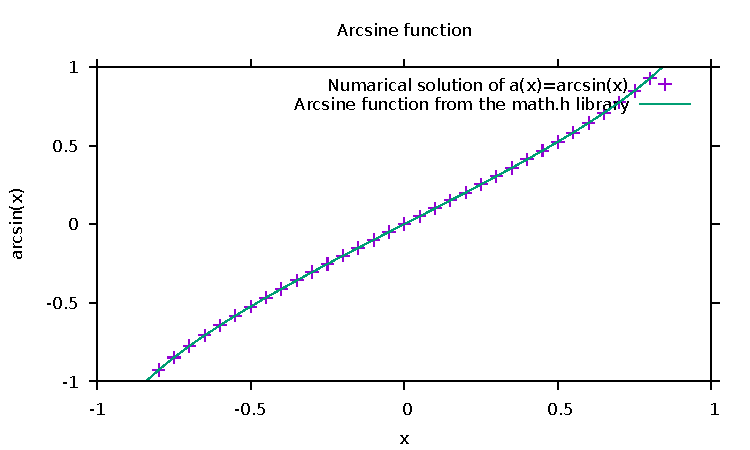
\includegraphics[width=\linewidth]{arcsin.pdf}
\caption{This figure shows the numerical solution of the arcsine function (plusses) together with the math.h arcsine function (line). }
\end{figure} 

It can be seen on figure \ref{fig:1} that the found numerical solution closely follown the math.h function. This result illustrates
the power of the root-finding algorythms as tools for numerical computation. 

\clearpage
\section{References}
\begin{thebibliography}{99}
\bibitem{wikiroots}
  Wikipedia article on the root finding algorythms\\
  \emph{WIKIPEDIA: ROOT-FINDING ALGORYTHM},\\
 \url{https://en.wikipedia.org/wiki/Root-finding_algorithm}\\
\\
\bibitem{GSL}
  Gnu Scientific Library page for the multidimensional root finding.\\
  \emph{GSL: MULTIDIMENSIONAL ROOT FINDING},\\
 \url{https://www.gnu.org/software/gsl/doc/html/multiroots.html}\\

\end{thebibliography}

\end{document}
